\documentclass{article}
\usepackage{amsmath}
\usepackage{enumerate}
\usepackage{hyperref}
\usepackage{graphicx}
%% --------------------------------------------------------------
\title{A very simple LaTeX}
\author{Tiep Vu}
\date{July 2016}

\begin{document}
\maketitle
\section{Problem} % (fold)
\label{sec:problem}
Given 3 real numbers $a, b, c$, solve the equation:
\begin{equation}
\label{eqn:problem}
    ax^2 + bx + c = 0 
\end{equation}
% section problem (end)

\section{Solution} % (fold)
\label{sec:solution}
\begin{enumerate}
	\item $a = 0$
	\begin{itemize}
		\item $b = 0, c \neq 0 \Rightarrow$ there is no solution for equation (\ref{eqn:problem}).
	\end{itemize}
	\item $a \neq 0 $. Let $\Delta = b^2 - 4ac$
\end{enumerate}
% section solution (end)

\section{Example} % (fold)
\label{sec:example}
Figure \ref{fig:graph1}
\begin{figure}[h]
\centering
	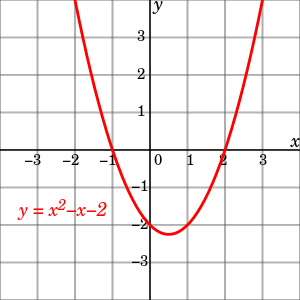
\includegraphics[scale = 0.3]{figs/fig1.png}
	\caption{The caption is here}
	\label{fig:graph1}
\end{figure}
% section example (end)

\section{Examples} % (fold)
\label{sec:examples}
Table \ref{tab:tb1}.
\begin{table}[h]
\centering
\caption{My caption}
\label{tab:tb1}
\begin{tabular}{|l|l|l|l|l|}
\hline
a & b  & c & x1 & x2 \\ \hline
1 & -4 & 3 & 1  & 3  \\ \hline
1 & -2 & 1 & 1  & 1  \\ \hline
\end{tabular}
\end{table}
% section examples (end)

\section{Citations} % (fold)
\label{sec:citations}
Tiep Vu \textit{et. al.} \cite{vu2015dfdl,vu2016histopathological}
% section citations (end)



\end{document}